%%%%%%%%%%%%%%%%%%%%%%%%%%%%%%%%%%%%%%%%%%%%%%%%%%%%%%%
% A template for Wiley article submissions.
% Developed by Overleaf. 
%
% Please note that whilst this template provides a 
% preview of the typeset manuscript for submission, it 
% will not necessarily be the final publication layout.
%
% Usage notes:
% The "blind" option will make anonymous all author, affiliation, correspondence and funding information.
% Use "num-refs" option for numerical citation and references style.
% Use "alpha-refs" option for author-year citation and references style.

%\documentclass[num-refs]{wiley-article}
%\documentclass[alpha-refs]{wiley-article}
%\documentclass[10pt]{elsarticle}
\documentclass{IEEEtran}
% Add additional packages here if required

\usepackage{siunitx}
\usepackage[font=footnotesize, justification = centering]{caption}
\usepackage[font=footnotesize]{subcaption}
\usepackage{algorithm}
\usepackage{algorithmicx}
\usepackage{amsmath}
\usepackage[noend]{algpseudocode}%no closing statement
\usepackage{algpseudocode}
\usepackage{graphicx}
% Update article type if known
%\papertype{Research Article}
% Include section in journal if known, otherwise delete


\title{Degree-based Balanced Clustering for Large-Scale Software Defined Networks}

% List abbreviations here, if any. Please note that it is preferred that abbreviations be defined at the first instance they appear in the text, rather than creating an abbreviations list.
%\abbrevs{ABC, a black cat; DEF, doesn't ever fret; GHI, goes home immediately.}

% Include full author names and degrees, when required by the journal.
% Use the \authfn to add symbols for additional footnotes and present addresses, if any. Usually start with 1 for notes about author contributions; then continuing with 2 etc if any author has a different present address.
%\author[1]{Talha Ibn Aziz}
%\author[1]{Shadman Protik}
%\author[1]{Md Sakhawat Hossen}
%\author[2]{Salimur Choudhury}
%\author[1]{Muhammad Mahbub Alam}

%\contrib[\authfn{1}]{Equally contributing authors.}

% Include full affiliation details for all authors

%\affil[1]{Department of Computer Science and Engineering, %Islamic University of Technology, Dhaka, Bangladesh}
%\affil[2]{Department of Computer Science, Lakehead University, %Thunder Bay, Ontario, Canada}

%\corraddress{Salimur Choudhury, Department of Computer %Science, Lakehead University, Thunder Bay, Ontario, Canada}
%\corremail{salimur.choudhury@lakeheadu.ca}

% Include the name of the author that should appear in the running header
%\runningauthor{Talha et al.}

\pagenumbering{gobble}

\setlength{\textfloatsep}{10pt plus 1.0pt minus 2.0pt}



\author{\IEEEauthorblockN{Talha Ibn Aziz\IEEEauthorrefmark{1}, Shadman Protik\IEEEauthorrefmark{1}, Md Sakhawat Hossen\IEEEauthorrefmark{1}, Salimur Choudhury\IEEEauthorrefmark{2} and Muhammad Mahbub Alam\IEEEauthorrefmark{1}}
	
	\IEEEauthorblockA{\IEEEauthorrefmark{1}Department of Computer Science and Engineering, Islamic University of Technology, Dhaka, Bangladesh \\  \IEEEauthorrefmark{2}Department of Computer Science, Lakehead University, Thunder Bay, Ontario, Canada} \\
	Email:  \IEEEauthorrefmark{1}talhaibnaziz@iut-dhaka.edu, \IEEEauthorrefmark{1}shadmanprotik@iut-dhaka.edu,
	\IEEEauthorrefmark{1}sakhawat@iut-dhaka.edu,
	\IEEEauthorrefmark{2}salimur.choudhury@lakeheadu.ca,  \IEEEauthorrefmark{1}mma@iut-dhaka.edu
}

\begin{document}
	
	\maketitle
	
	
	
	\begin{abstract}
		
		\noindent 
		The Controller Placement Problem (CPP), in Software Defined Networks (SDNs), deals with placing an optimal number of controllers. The CPP aims to maximize the network throughput and minimize different latencies like flow-setup latency and route-synchronization latency. In recent years, many solutions to the CPP have been proposed-- some approaches work with a single parameter like the average propagation delay of a network, reliability, load balancing, etc., while some other approaches provide exhaustive solutions which optimize multiple parameters. However, very few researches propose non-exhaustive solutions which simultaneously optimize more than one parameter. We propose a novel controller placement algorithm which clusters the SDNs in polynomial time complexity. Our proposed algorithm Degree-based Balanced Clustering (DBC) minimizes overall flow-setup latency as well as route-synchronization latency and balances the loads of the controllers at the same time. DBC divides a network into several clusters, places a controller in each cluster, and also selects an optimal number of controllers. Simulation results suggest that DBC outperforms existing state-of-the-art algorithms in terms of different latencies and also performs load balancing among the controllers.
		
		\begin{IEEEkeywords}
			CPP, SDN, latency, controller, load-balancing
		\end{IEEEkeywords}
		
	\end{abstract}
	
	
	
	\section{Introduction}
	
	Software Defined Networks (SDNs) decouple the traditional protocol stack into control plane and data plane. The control plane consists of controllers which take the routing decisions and relay this information to the data plane. The data plane is the collection of switches which forward the data according to the routing decisions provided by the control plane. The initial design of SDN included a single controller in the control plane \cite{greene2009tr10}. However, even for moderate-sized networks, a bottleneck is created due to heavy traffic concentrated at the controller. Furthermore, problems like scalability and reliability surface as network sizes increase \cite{scalability2013dixit, scalability2013yeganeh}. In order to deal with these problems, many researches propose multiple controllers \cite{whycpp2010, whycpp2013, whycpp2014, haque2016wireless}, which results in the emergence of the Controller Placement Problem (CPP). The CPP deals with placing a minimal number of controllers in the SDNs, with an aim to address the above mentioned problems.
	
	A solution to the CPP is to select an optimal number of controllers, to place them in the best possible locations, and to assign them switches in an optimal way \cite{sdnwan2014, sdnlange2015}. In addition, there are multiple constraints that need to be satisfied-- minimizing the latency among switches and controllers, maximizing reliability and resilience, and minimizing deployment cost as well as energy consumption, which results in an NP-Hard problem. Despite the complications, in recent years, several solutions have been proposed to address the CPP \cite{cppsurvey2017, cppsurvey2018, cpp2018sudheera, sdnsurvey2017, sdniotsurvey2016}, where some of them deal with optimizing a particular constraint like latency or reliability, while some others introduce a compound metric to address two or more constraints.
	
	Heller et. al. \cite{cpp2012heller} calculate the average and worst case latencies to place controllers and mention that multiple controllers are more significant in ensuring fault-tolerance than to minimize latency. Yao et. al. \cite{yao2015controller} propose dynamic scheduling strategies based on changing flows to manage controllers aiming to balance their loads. Hu et. al. \cite{hu2013reliability} propose multiple algorithms for reliability-aware controller placement. Zhang et. al. \cite{zhang2011resilience} use a min-cut based graph partitioning algorithm to maximize resilience of SDNs and compare the algorithm with greedy approaches. In \cite{lange2015heuristic}, Lange et. al. propose POCO (Pareto-based Optimal COntroller placement), which represents the CPP as a combinatorial optimization problem. POCO exhaustively iterates all possible combinations as viable solutions to optimize multiple metrics and uses heuristics-based PSA (Pareto Simulated Annealing) to improve the computational complexity at the cost of accuracy. Sallahi et. al. \cite{sallahi2015optimal} propose a mathematical model for optimal controller placement considering the cost of installing controllers, loads of the controllers and path setup latency. Exhaustive solutions like \cite{lange2015heuristic, sallahi2015optimal} can give optimal solutions, however, their computational complexities are very high.
	
	Liao et. al. \cite{dbcp2017} propose two faster algorithms Density Based Controller Placement (DBCP) and Capacitated-DBCP (CDBCP) where DBCP minimizes overall latency based on the local density of the nodes and CDBCP balances the load of the controllers. However, they work separately on the given network to perform controller placement and to balance the load of the controllers. To the best of our knowledge, no other methods minimize overall latency and perform load balancing simultaneously, while clustering SDNs in polynomial time complexity. In this paper, we place minimum (optimal) number of controllers in a SDN to minimize the followings:
	\begin{enumerate}
		\item \textbf{Flow setup latency:} When a switch receives a packet for which no path exists, the flow-setup procedure is initiated. The latency introduced by this procedure is the maximum delay required to set the path (and also to inform the intermediate switches) for the flow.
		\item \textbf{Route synchronization latency:} When there is a change in the network, routes are changed, and all the controllers are updated (in sync) about the changes. This latency deals with controller-to-controller latency.
		\item \textbf{Load of a controller:} The volume of control traffic and processing that the switches impose on the controllers.
	\end{enumerate}
	
	This requires placing the controllers in a way that minimizes both the average controller-to-switch and average controller-to-controller latencies and limits the load of the controllers. In this paper, we propose and develop an algorithm named Degree-based Balanced Clustering (DBC) to achieve the above with a careful selection of controllers. Simulation results suggest that our proposed algorithm DBC outperforms the state-of-the-art algorithms in terms of overall latency and load balancing. We also observe that the above criteria can be achieved if we can divide the SDN into $k$ balanced clusters.
	
	The rest of the paper is organized as follows-- we provide our problem formulation along with some assumptions in Section \ref{sysMod}, a detailed description of our proposed mechanism in Section \ref{proposedalgo}, we present simulation results and performance evaluation in Section \ref{performance}, and we conclude in Section \ref{conclusion}.
	
	
	
	\section{System Model and Assumptions} \label{sysMod}
	
	We consider that the network is a bi-directional graph $G=(S, L)$, where, the set of nodes $S$ represent the switches and the set of edges $L$ represent the links between the switches. The edges can be either weighted or unweighted based on the requirements. We cluster the graph $G$ into multiple sub-networks such that, each sub-network is a disjoint set of switches. There cannot be any common switch between two sub-networks, and all of the switches of the network must fall into a sub-network, where each sub-network will have one and only one controller. Accordingly, if we assume that the network is partitioned into $k$ sub-networks, then there will be $k$ controllers and each sub-network will be a disjoint set of switches containing a single controller. For simplicity we make the following four assumptions:
	\begin{enumerate}
		\item The transmission delay of each control packet is identical and negligible.
		\item The propagation delay, queuing delay and processing delay of each switch is identical.
		\item The load imposed by each switch is fixed.
		\item The controller can only replace a switch and cannot be placed in any other locations.
	\end{enumerate}
	Under these assumptions, our objective is to minimize the flow-setup latency, the inter-controller distances and the controller-to-switch distances in each sub-network, all of which are measured in hop counts. We also aim to balance the load of each controller, which is the number of switches assigned to each controller.
	
	\section{Proposed Mechanism} \label{proposedalgo}
	
	We propose a solution to the CPP referred to as Degree-based Balanced Clustering (DBC) for SDN. The proposed mechanism divides the networks into $k$-clusters, assigns a controller to each cluster, and finally, finds the minimum value of $k$ for the network which obtains the minimum latency. In the sequel, we explain the mechanism in detail.
	
	\subsection{Cluster Formation}
	
	The cluster formation mechanism divides the network into $k$ clusters (sub-networks), when $k$ is given. It finds the $k$ cluster heads first and then, assigns each of the nodes to exactly one sub-network. The clustering mechanism deals with two goals--
	\begin{itemize}
		\item Equal load on the controllers, which requires equal number of nodes in each cluster. We assume that the switches have equal load.
		\item Minimum intra-cluster distances between the nodes and cluster heads, which requires direct (or shortest path) connectivity of the nodes and the cluster heads.
	\end{itemize}
	
	The first goal demands more clusters in the denser part of the network, whereas, the second goal demands the nodes with maximum direct connections with the switches to be the cluster heads. Accordingly, a cluster head should have the highest connectivity among all the switches of its cluster so that maximum number of nodes can be reached with minimum delay. Both the two goals can be achieved if the clustering is done based on degree of the node.
	
	A degree based solution to the second goal suggests selecting $k$ nodes with highest degrees as the cluster heads of the network. This solution ensures minimization of intra-cluster delay when the highest degree nodes are uniformly distributed (well separated). However, in typical networks, the higher degree nodes are situated in the same locality of the network. Consequently, the dense regions of the network are dominated by most of the cluster heads, and the clusters formed are not balanced in terms of load (first goal). Therefore, the cluster heads need to be a certain distance apart from each other, which we define as the minimum inter cluster head distance, $T_d$. The threshold, $T_d$, simultaneously maintains a fixed cluster head separation and balances the load of the network.
	
	
	%The controller-to-switch latency of a network improves when the switches are in close proximity of the controller and the controller-to-controller latency depends on the latencies of the paths between controllers. Therefore, to minimize total delay, the network needs to be clustered in such a way that both intra-cluster and inter-cluster distances are minimized. Moreover, the load of the network should be evenly distributed to avoid overburdening any controller. Under these constraints, we can assume that, the sub-networks will ideally have minimum cluster radii and similar number of nodes. Having minimum cluster radii will simultaneously reduce intra-cluster and inter-cluster distances, while having similar cluster sizes will balance the load on each controller as much as possible.
	
	
	The cluster head separation dictates the number of switches in a cluster, which should be roughly $|S|/k$ for a balanced cluster. Initially, for $T_d=1$ hop count, the nodes in the cluster are the cluster head itself and one-hop neighbors of the cluster head. Consequently, in an average case scenario, the total number of nodes is $1+AvgDeg$, where $AvgDeg$ denotes the average node degree of the network. According to graph theory, each link simultaneously increments the degree of two switches by one, which implies that, the summation of the node degrees of a network is $2\times |L|$ and the average node degree is $\frac{2\times |L|}{|S|}$.
	
	We denote the total number of nodes in the periphery of the cluster as $boundary$. Initially, $boundary=AvgDeg$, as the cluster consists of a cluster head at the center and its one-hop neighbors on the border which is equivalent to $AvgDeg$ nodes on average. Each boundary node is again connected to approximately $AvgDeg$ number of nodes including the cluster head itself. Therefore, omitting the cluster head, for every increment of the value of $T_d$, the number of nodes in the cluster increases following the given formula,
	\begin{equation} \label{eqn:clusterIncrease}
	boundary = boundary \times (AvgDeg - 1)
	\end{equation}
	
	When the total number of nodes in the cluster exceeds $|S|/k$ nodes, we terminate the increment process. The value of $T_d$ thus obtained is the threshold distance or cluster separation of a balanced cluster.
	
	In DBC, we sort the nodes according to descending value of node degree (line 1 of algorithm \ref{algo:dbc}) and select the node with highest degree as first cluster head. We select a cluster head from the remaining nodes, only if it is at least $T_d$ distance away from the selected cluster heads, otherwise we omit it, and move on to the next node in the sorted list. The region of the selected node may be sparser than other parts of the network. In order to take this into account, we multiply the threshold $T_d$ with a degree ratio (line 13 of algorithm \ref{algo:dbc}), which is the maximum degree of the network divided by the degree of the selected node. The degree ratio ranges the $T_d$ value according to the density of the node, if the degree of the node is less, the density is lower. Accordingly, the ratio has a higher value $(\frac{Maximum~Degree}{degree~of~selected~node}>1)$ and increases the cluster separation threshold to include more nodes than in a denser region. However, if $k$ cluster heads cannot be selected in this way, we select the remaining cluster heads only based on degree and ignore their distance from other cluster heads. Consequently, all the remaining nodes are assigned to the cluster of the nearest cluster head and $k$ clusters are formed.
	
	\subsection{Controller Selection}
	After completion of the clustering process we initiate a controller selection process. The total delay of a network depends on both controller-to-controller latency and controller-to-switch latency. The controller-to-switch latency of a network improves when the switches are in close proximity of the controller and the controller-to-controller latency depends on the latencies of the paths between controllers. Although the cluster head has high intra cluster connectivity, inter cluster distance also needs to be taken into account. Considering both intra cluster and inter cluster distances (which refers to controller-to-controller latency), the cluster may or may not be the controller. Accordingly, we define $\tau(s)$ to be the controller selection function of switch $s$, which comprises its intra-cluster distance $\phi(s)$ and inter-cluster distance $\sigma(s)$ values. The intra-cluster distance can be calculated as the average distance from the switch $s$ of cluster $S_i$ to the other nodes of $S_i$ \cite{dbcp2017},
	\begin{equation} \label{eqn:intra}
	\phi(s) = \frac{1}{|S_i|-1}\sum_{u\in S_i} dis(s,u)
	\end{equation}
	
	here, $u$ represents any other switch in the same cluster $S_i$, as switch $s$ and $|S_i|$ is the total number of switches in $S_i$. The component $\phi(s)$ corresponds to the controller-to-switch latency and $dis(s,u)$ is the shortest path distance of $s$ from $u$.
	
	The inter-cluster distance, which is the other component of total latency $\tau$ corresponds to the controller-to-controller latency. However, we cannot calculate inter-controller distances before the controller selection process as there are no controllers to begin with. Hence, we calculate $\sigma(s)$ for a switch $s$ of cluster $S_i$, as the average distance of $s$ from all other nodes of the network that are not in $S_i$ \cite{dbcp2017},
	\begin{equation} \label{eqn:inter}
	\sigma(s) = \frac{1}{|S-S_i|}\sum_{v\in (S-S_i)} dis(s,v)
	\end{equation}
	
	here, $v$ denotes the switches that belong to  network $S$ but does not belong to sub-network $S_i$. The set of all nodes except sub-network $S_i$, is denoted by $S-S_i$.
	
	The controller selection function $\tau(s)$ can be defined as the direct summation of the component latencies $\phi(s)$ and $\sigma(s)$. Although, this assigns equal weight to the inter-cluster latency and intra-cluster latency, the inter-cluster latency dominates overall latency as controller-to-controller distance is usually greater than controller-to-switch distance. We introduce a weight variable $\alpha$ to control this dominance and give the user the freedom to emphasize on any component as per requirement,
	\begin{equation} \label{eqn:totlat}
	\tau(s) = \alpha \times \phi(s) + (1-\alpha) \times \sigma(s)
	\end{equation}
	
	In our experiments, we set the values of $\alpha$ as $0.5$. As a result, both components contribute equally in the controller selection process. The pseudocode of our proposed method is given below (algorithm \ref{algo:dbc}). The algorithm takes the network switches, $S$, links, $L$, and number of clusters, $k$, as input, and returns $k$ optimal network clusters $C_1,C_2,...,C_k$ and the set of $Controllers$ for the clusters. The worst case time complexity of the sorting (line 1 of algorithm \ref{algo:dbc}) is $O(|S|\log(|S|))$, the cluster head separation determination (line 11-19) is $O(|S|)$, and the controller selection (27-31) is $O(|S|^2)$. Consequently, the over all worst case time complexity of DBC is $O(|S|^2)$.
	
	\begin{algorithm}
		\caption{: Degree-based Balanced Clustering (DBC)}\label{algo:dbc}
		\begin{algorithmic}[1]
			\Procedure{DBC}{} \\
			\textbf{input:} $k,S,L$ \\
			Sort $S$ in descending order of degree \\
			Initialize $AvgDeg := \frac{2\times |L|}{|S|}$ and $boundary:=AvgDeg$ \\
			Initialize $limit:=1+AvgDeg$ \\
			Initialize threshold distance $T_d := 0$ \\
			Initialize $clusterHeads := \emptyset$
			\While{$limit<(|S|/k)$}
			\State $boundary=boundary\times (AvgDeg-1)$
			\State $limit:=limit + boundary$; $T_d:=T_d+1$
			\EndWhile
			\For {each switch s in $S$}
			\State $adjT_d=T_d\times \frac{max~degree}{degree~of~s}$
			\If {$clusterHeads = \emptyset$}
			\State $clusterHeads.add(s)$
			\ElsIf {$clusterHeads.size = k$} break
			\ElsIf {$dis(s,clusterHeads)<adjT_d$}
			\State continue
			\Else
			\State $clusterHeads.add(s)$
			\EndIf
			\EndFor
			\If {$clusterHeads.size<k$}
			\State Select remaining $clusterHeads$ with max degree
			\EndIf \\
			Initialize clusters $C_1,C_2,...,C_{k}$ as $\emptyset$ \\
			Initialize $Controllers:=\emptyset$
			\For {each cluster $C_i$}
			\State $C_i:={clusterHeads[i]}$
			\State $C_i:=C_i \cup \{nearest~nodes~of~C_i\}$
			\EndFor
			\For {each cluster $C_i$}
			\For {all $s\in C_i$}
			\State Calculate $\phi(s)$ and $\sigma(s)$
			\State $\tau(s) := \alpha \times \phi(s) + (1-\alpha) \times \sigma(s)$
			\EndFor
			\State $Controllers.add(node~with~min(\tau(s)))$
			\EndFor \\
			\textbf{output:} $Controllers$ \\
			\textbf{output:} $C_1,C_2,...,C_{k}$
			\EndProcedure
		\end{algorithmic}
	\end{algorithm}
	
	\subsection{Optimum k Selection} \label{optimumK}
	We evaluate the performance of each clustering using its average flow setup latency and denote this evaluation function by $\Omega(S)$ for a network $S$. When a data packet arrives at a switch $s_i$, for which no entry exists in its flow table, the switch forwards the packet encapsulated in a query message to its controller $c_i$. The controller decides the path for the packet and notifies the other switches of the path about the new flow rule, through their controllers. The switches on the path from $s_i$ to destination $s_d$, may have different controllers. Consequently, the generated control packet containing the new route, needs to be forwarded to the controllers, which in turn will instruct the concerned switches to update their flow tables. Since the process is parallel, the path setup latency is dominated by the maximum of the sum of the distances from the corresponding controller of the source $c_i$, to controller $c_j$ of any intermediate node $s_j$, and from $c_j$ to $s_j$. Therefore, the evaluation function can be calculated as the average setup latency of all possible switch pairs \cite{dbcp2017},
	\begin{equation} \label{eqn:setupLatency}
	\begin{split}
	\Omega(S) = &\frac{2}{|S|\times |S-1|}\sum_{s_i,s_d\in S} \{dis(s_i,c_i)+\\ &\max_{s_j\in path_{i,d}}\left(dis(c_i,c_j)+dis(c_j,s_j) \right) \}
	\end{split}
	\end{equation}
	
	here, $path_{i,d}$ is the shortest path from source $s_i$ to destination $s_d$. We use this function as the performance evaluation metric in section \ref{performance}.
	
	We increment $k$ (starts at 1) and apply DBC repeatedly until the improvement in terms of $\Omega(S)$ is negligible. We define the improvement ratio or termination criteria $\xi$ as follows,
	\begin{equation} \label{eqn:optimalK}
	\gamma = \frac{(\Omega_{old~k}(S)-\Omega_{new~k})/\Omega_{old~k}}{new~k-old~k}
	\end{equation}
	
	here, $old~k$ is the previous value of $k$ and $new~k$ is the incremented value. In our simulations we notice a sharp drop in the value of $\gamma$ after a certain number of increments.
	
	\section{Performance Evaluation} \label{performance}
	
	\subsection{Simulation Environment} \label{simulationEnv}
	We developed a simulation environment using C++ (High-level language) which takes the number of nodes and connections between each node as input and clusters the network. We use randomly generated networks with different numbers of switches starting from 40 to 100, at regular intervals of 10. There are 10 different datasets for each interval, giving a total of 70 different networks. The link to switch ratio is from 1.3 to 1.45 to keep the networks considerably sparse (similar to current worldwide networks). The simulation environment and selected 70 networks are same for both our algorithm and DBCP. The networks do not contain any self-loops or multiple links between two switches but may have cycles. The average number of edges of the scenarios are 54, 66.7, 81.4, 99.3, 111.2, 125.5 and 138.9 respectively.
	%\begin{table}
	%	\begin{center}
	%		\textbf{\caption{Randomized Networks used as Input} \label{table:networks}}
	%		\begin{tabular}{|l|c|c|l|}
	%			\hline
	%			Scenario & Nodes & Edges & Edge/Node \\
	%			\hline
	%			1 & 40 & 54 & 1.35\\
	%			2 & 50 & 66.7 & 1.334\\
	%			3 & 60 & 81.4 & 1.35667\\
	%			4 & 70 & 99.3 & 1.41857\\
	%			5 & 80 & 111.2 & 1.39\\
	%			6 & 90 & 125.5 & 1.39444\\
	%			7 & 100 & 138.9 & 1.389\\
	%			\hline
	%		\end{tabular}
	%	\end{center}
	%\end{table}
	
	\subsection{Performance Metrics}
	We use various performance metrics to study and evaluate different characteristics of SDNs like inter-controller latency, controller-to-switch latency, and overall network switch to switch latency. We calculate the average inter-controller latency as follows,
	\begin{equation} \label{eqn:interController}
	\eta^{interController} = \frac{1}{k\times(k-1)}\sum_{1\le i,j \le k, i\ne j}dis(c_i,c_j)
	\end{equation}
	
	where, $c_i$ and $c_j$ are controllers of the SDN. We evaluate the controller-to-switch latency using the following equation,
	\begin{equation} \label{eqn:controllerSwitch}
	\eta^{controllerSwitch} = \frac{1}{k}\sum_{i=1}^{k}\bigg[\frac{1}{|S_i-1|}\sum_{u\in S_i}dis(c_i,u)\bigg]
	\end{equation}
	
	here, $S_i$ is the $i^{th}$ sub-network, $c_i$ is the controller and $u$, the switch of $S_i$. Both $\eta^{controllerSwitch}$ and $\eta^{interController}$ consider the shortest distance from the controller to any other controller or switch. However, for setup of a new route, the switch sends a packet to the controller, which decides the new route and relays the information to other concerned controllers and switches. We calculate this latency using the equation \ref{eqn:setupLatency} which has been discussed in section \ref{optimumK}.
	
	We also evaluate the load of each controller, considering that all switches have the same load. For an ideal clustering of an SDN, the number of nodes per cluster should be $|S|/k$. However, the actual clustering may vary from the ideal case, which can be considered as the deviation. Accordingly, the least deviation from the ideal case is the most balanced in terms of load. The deviation can be denoted by,
	\begin{equation} \label{eqn:deviation}
	\eta^{loadDeviation}=\frac{1}{k}\max_{i=1}^{k}(||S_i|-|S|/k|)
	\end{equation}
	
	where, $|S_i|$ is the number of nodes in the $i^{th}$ sub-network and $|S|$ is the total number of nodes in the network.
	
	\subsection{Simulation Results} \label{results}
	We validate our proposed method through extensive simulations. We compare our proposed algorithm with DBCP \cite{dbcp2017} in terms of flow-setup latency, average inter-controller latency, average controller-to-switch latency and load balancing. To compare flow-setup latency, we use the value of $k$ provided by DBCP to cluster the network and place the controllers. We plot the flow setup latencies as the average of the 10 instances in Fig. \ref{fig:dbcVsdbcp1}. We calculate the setup latency of each instance using equation \ref{eqn:setupLatency} of section \ref{optimumK}.
	
	\begin{figure}
		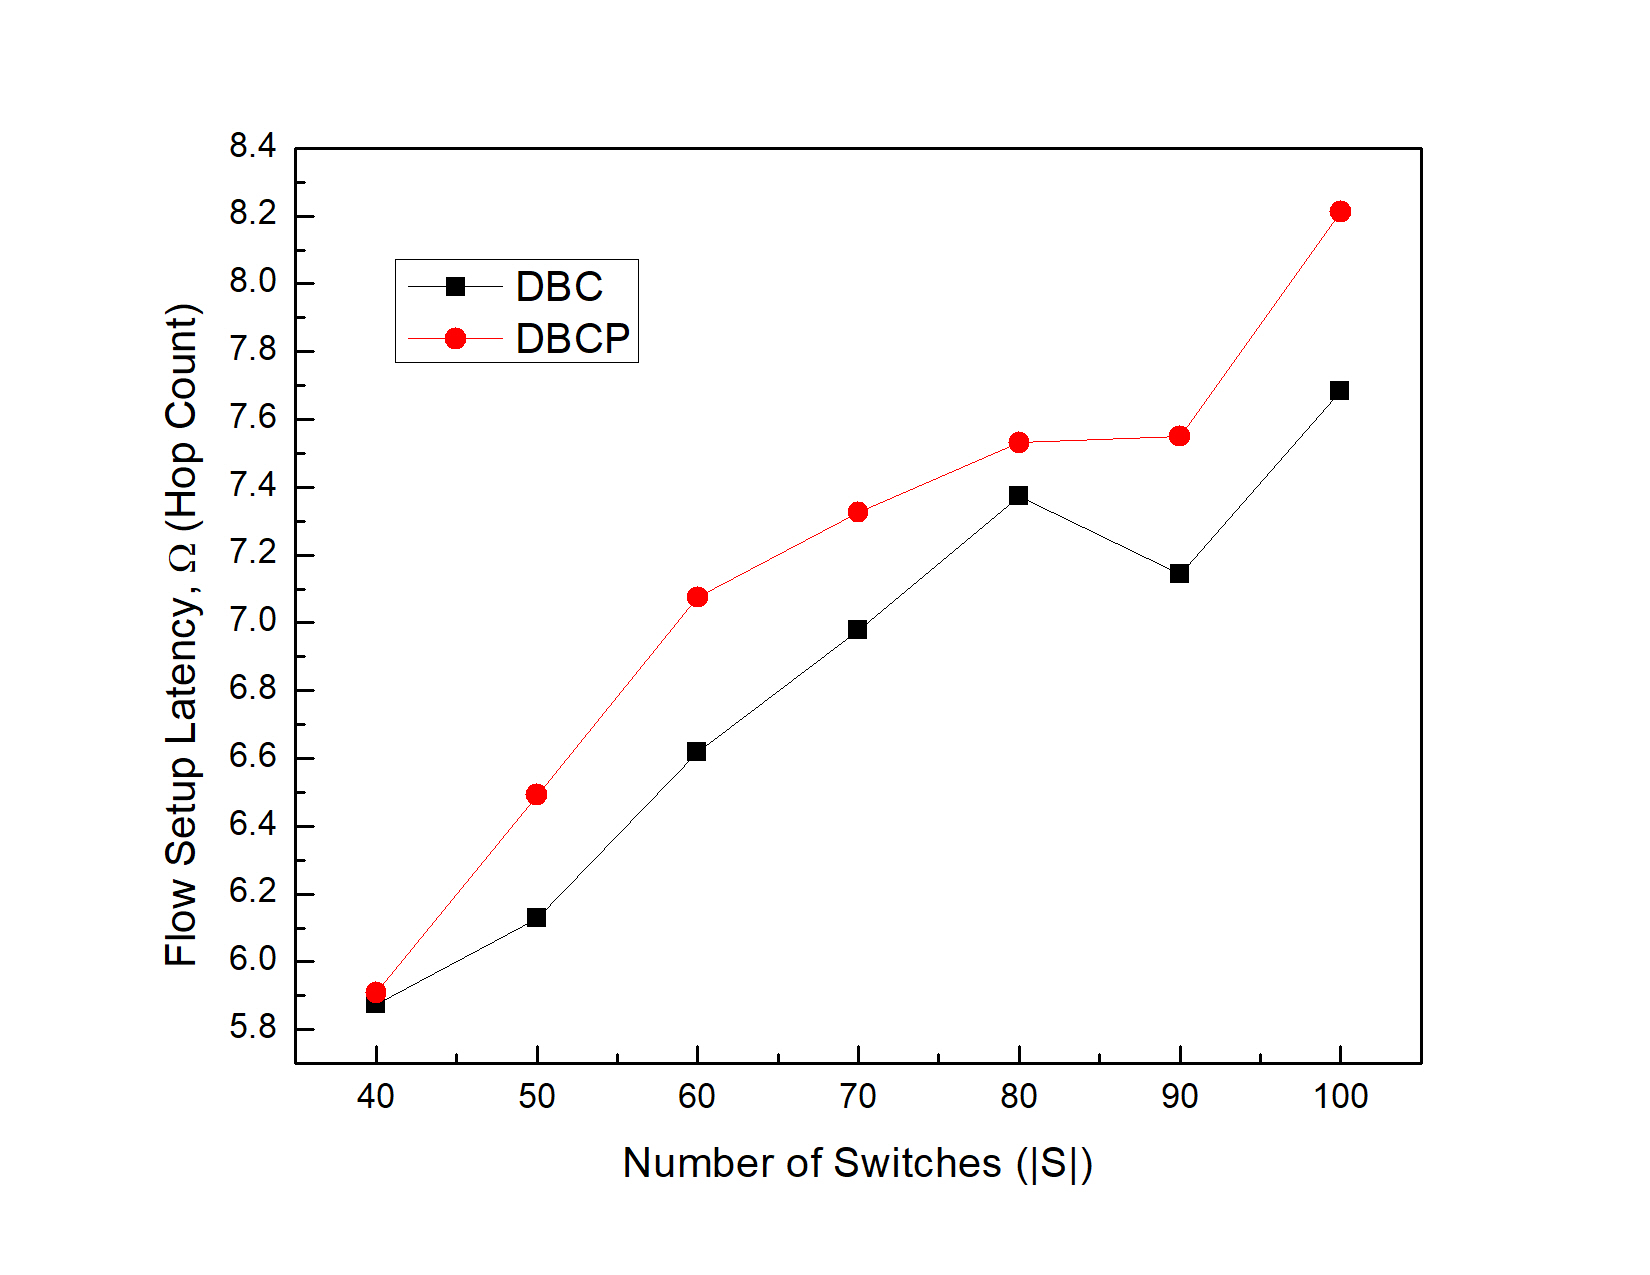
\includegraphics[width=\linewidth]{Figures/dbc_vs_dbcp1.jpg}
		\caption{Comparison of flow-setup latency between DBC and DBCP using the value of $k$ provided by DBCP}
		\label{fig:dbcVsdbcp1}
		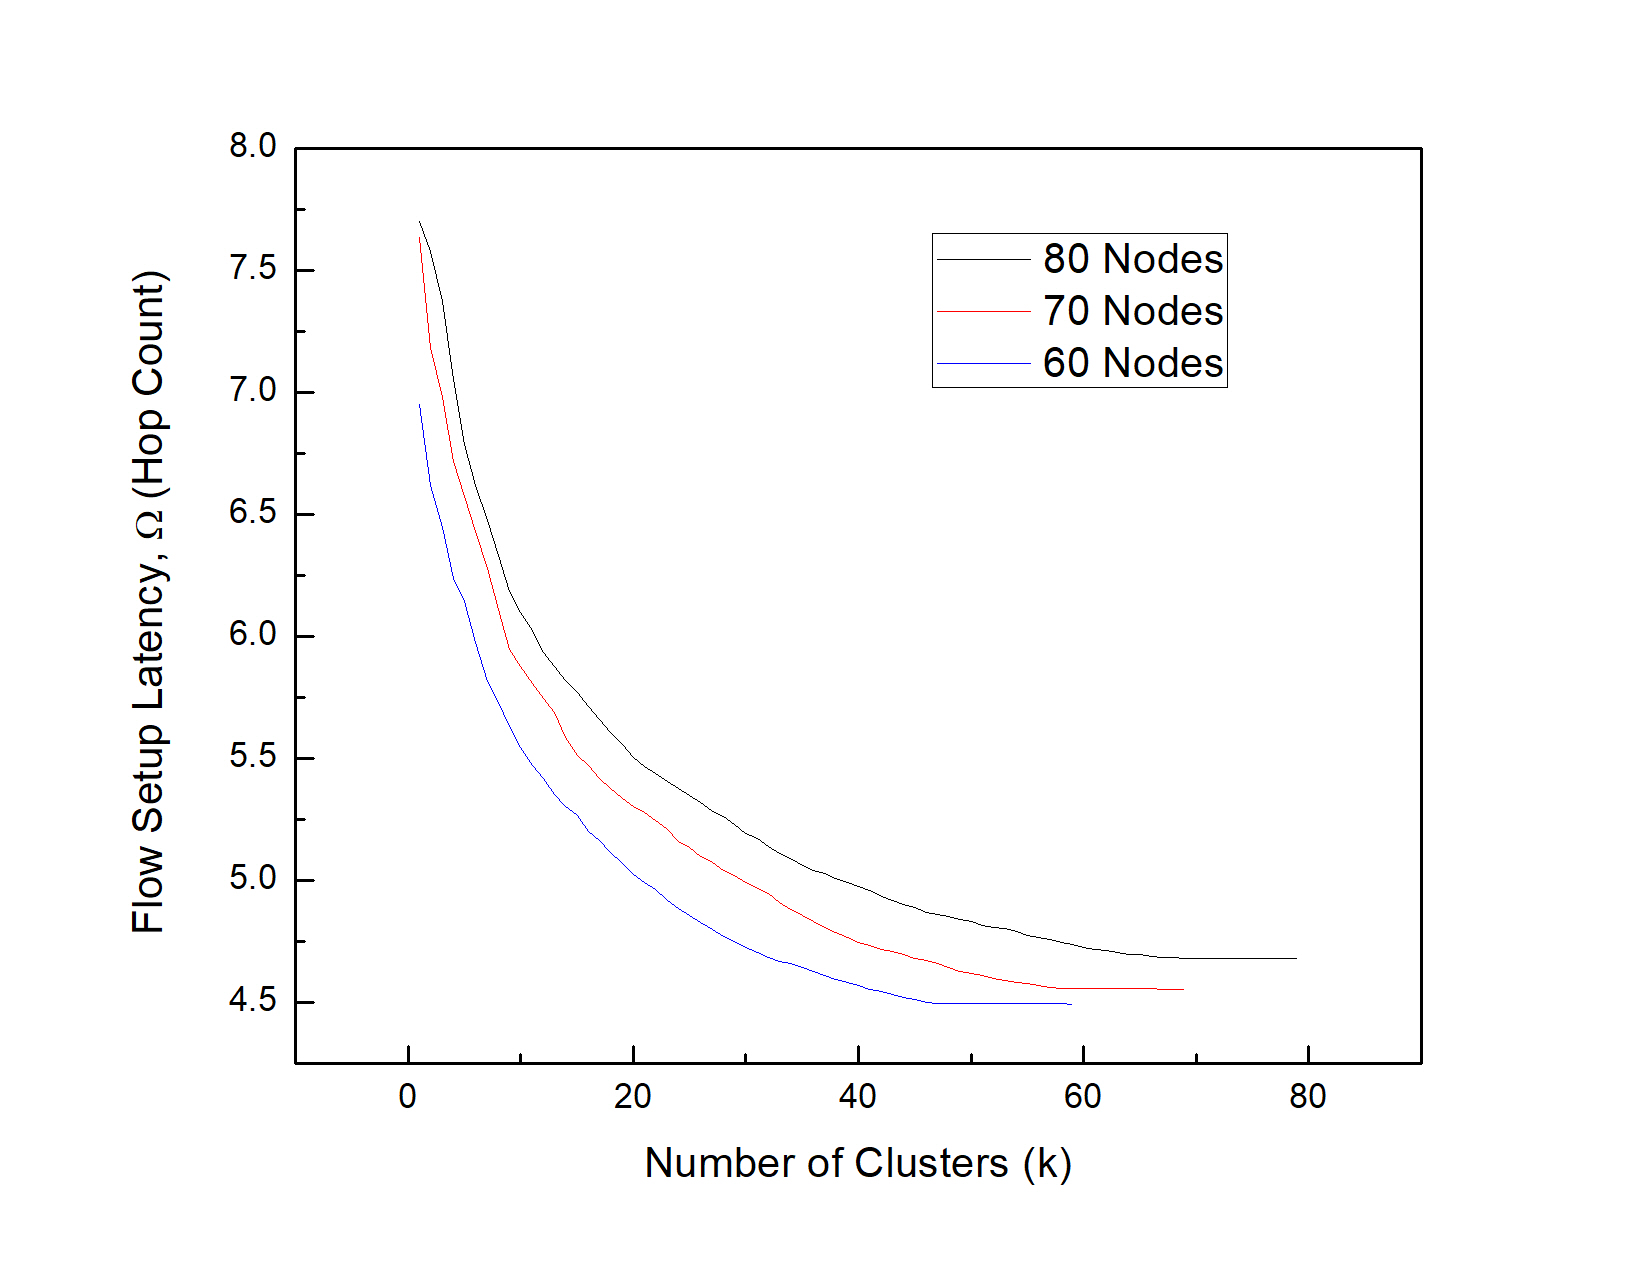
\includegraphics[width=\linewidth]{Figures/kGraph.jpg}
		\caption{Decreasing flow-setup latency with respect to increasing cluster numbers ($k$) for networks containing 60, 70, and 80 nodes}
		\label{fig:kGraph}
	\end{figure}
	Fig. \ref{fig:dbcVsdbcp1} shows that DBC outperforms DBCP, however, for smaller networks the difference in performance is less (when number of switches is 40). In all other cases, the difference in performance is noticeable. We can observe that, for both the algorithms, the latency values ($\Omega$) increase with the number of switches in the network. However, when the number of nodes is 90, the latency for both of the algorithms decrease slightly due to inconsistency of underlying topology.
	
	In Fig. \ref{fig:kGraph}, we plot the flow-setup latency with respect to controller number $k$ for networks containing 60, 70, and 80 switches. For greater values of k, the rate of improvement in terms of flow-setup latency is less as the placement of more controllers does not decrease the controller-to-switch distances significantly. We use this property to define an optimum $k$ selection function (equation \ref{eqn:optimalK}), using which we terminate the process when the improvement ratio, $\gamma$, is negligible (meaning negligible improvement). We notice a sharp drop in improvement rate at higher values of $k$ where $\gamma > 0.05$, so we set the terminating threshold at $0.05$. Accordingly, we plot the flow-setup latencies for the new values of $k$ in Fig. \ref{fig:dbcVsdbcp2}, where, we observe that our algorithm is more consistent than previously selected $k$ values which were selected by DBCP. The flow-setup latencies have also improved, and the number of controllers have decreased (Fig. \ref{fig:barDiagram}). The number of controllers is comparatively less as the clusters are more balanced due to the consideration of a standard cluster-separation $T_d$. As a result of the formation of such clusters, the controller-switch and controller-controller distances are minimized. Consequently, in all the scenarios, DBC outperforms DBCP in terms of both flow-setup latency and minimum number of controllers.
	
	\begin{figure}
		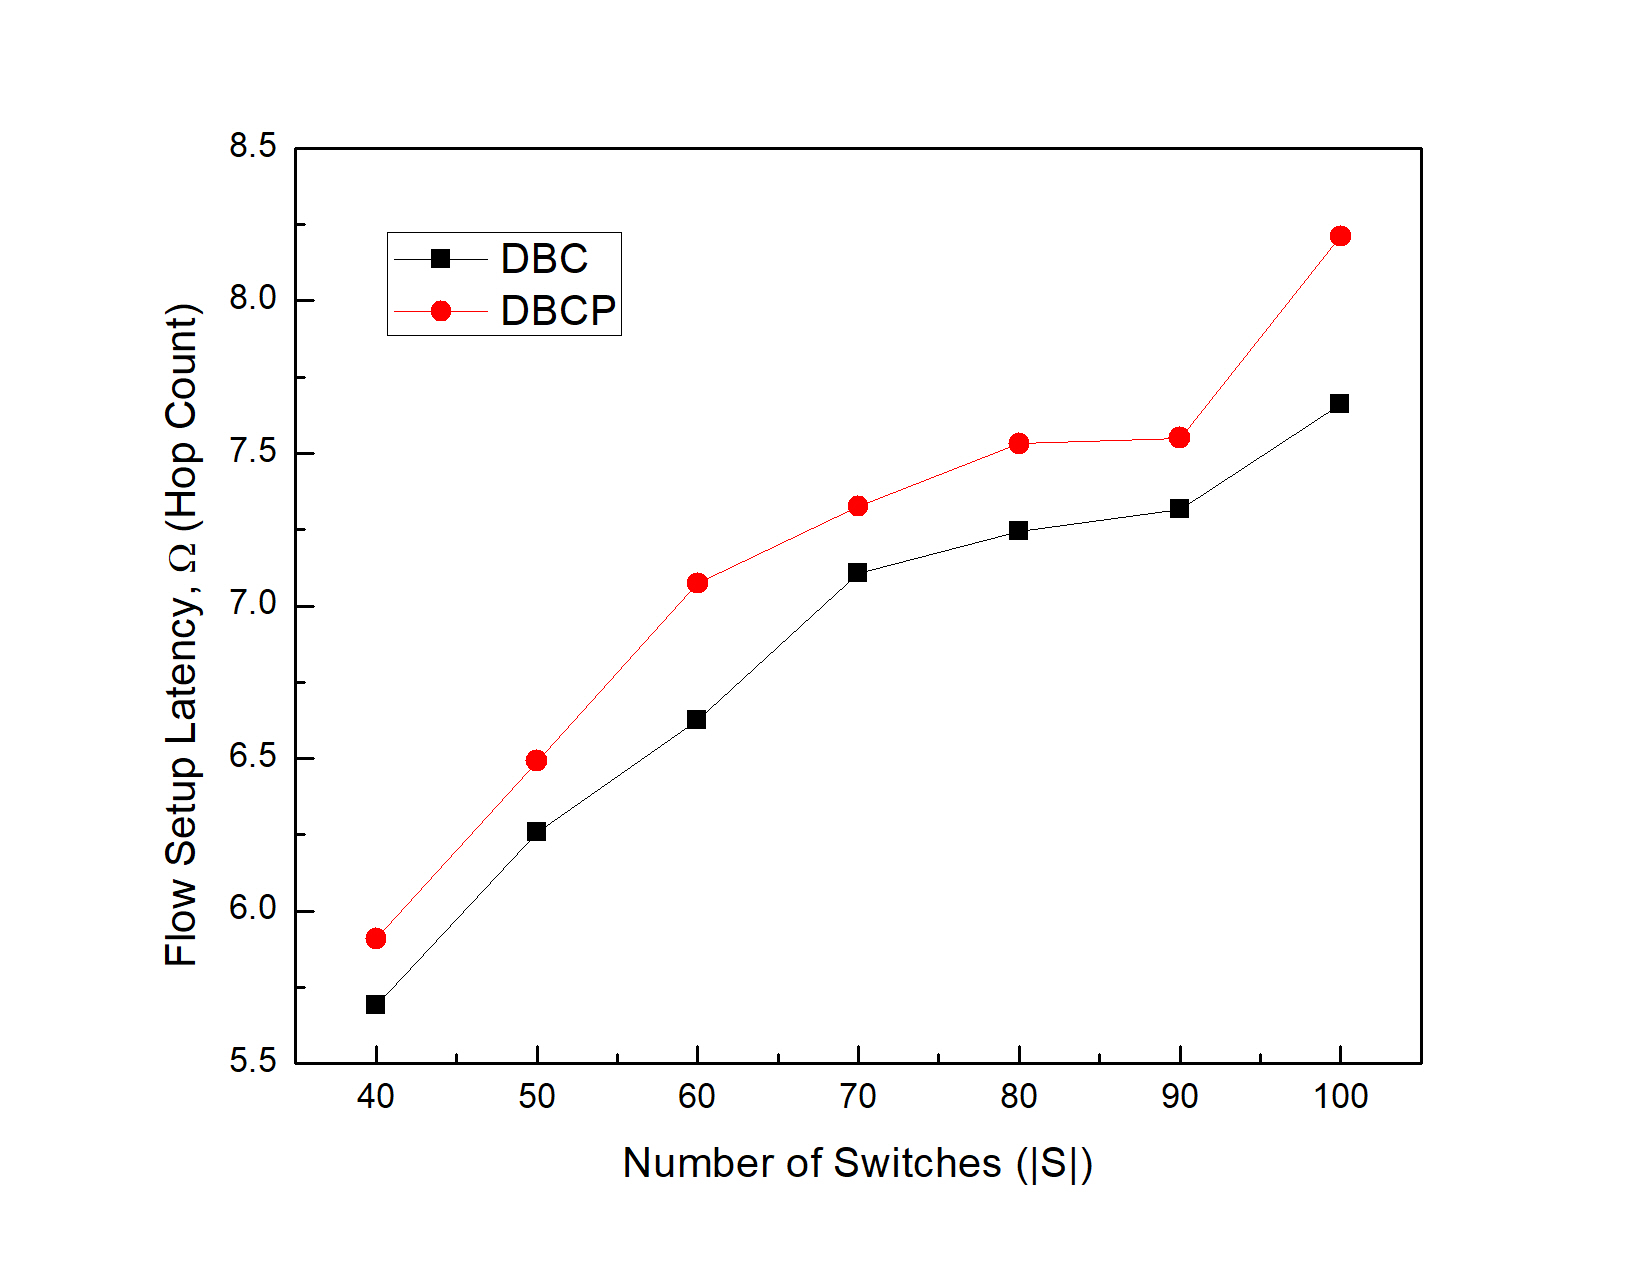
\includegraphics[width=\linewidth]{Figures/dbc_vs_dbcp2.jpg}
		\caption{Comparison between DBC and DBCP in terms of flow-latency, $\Omega$}
		\label{fig:dbcVsdbcp2}
		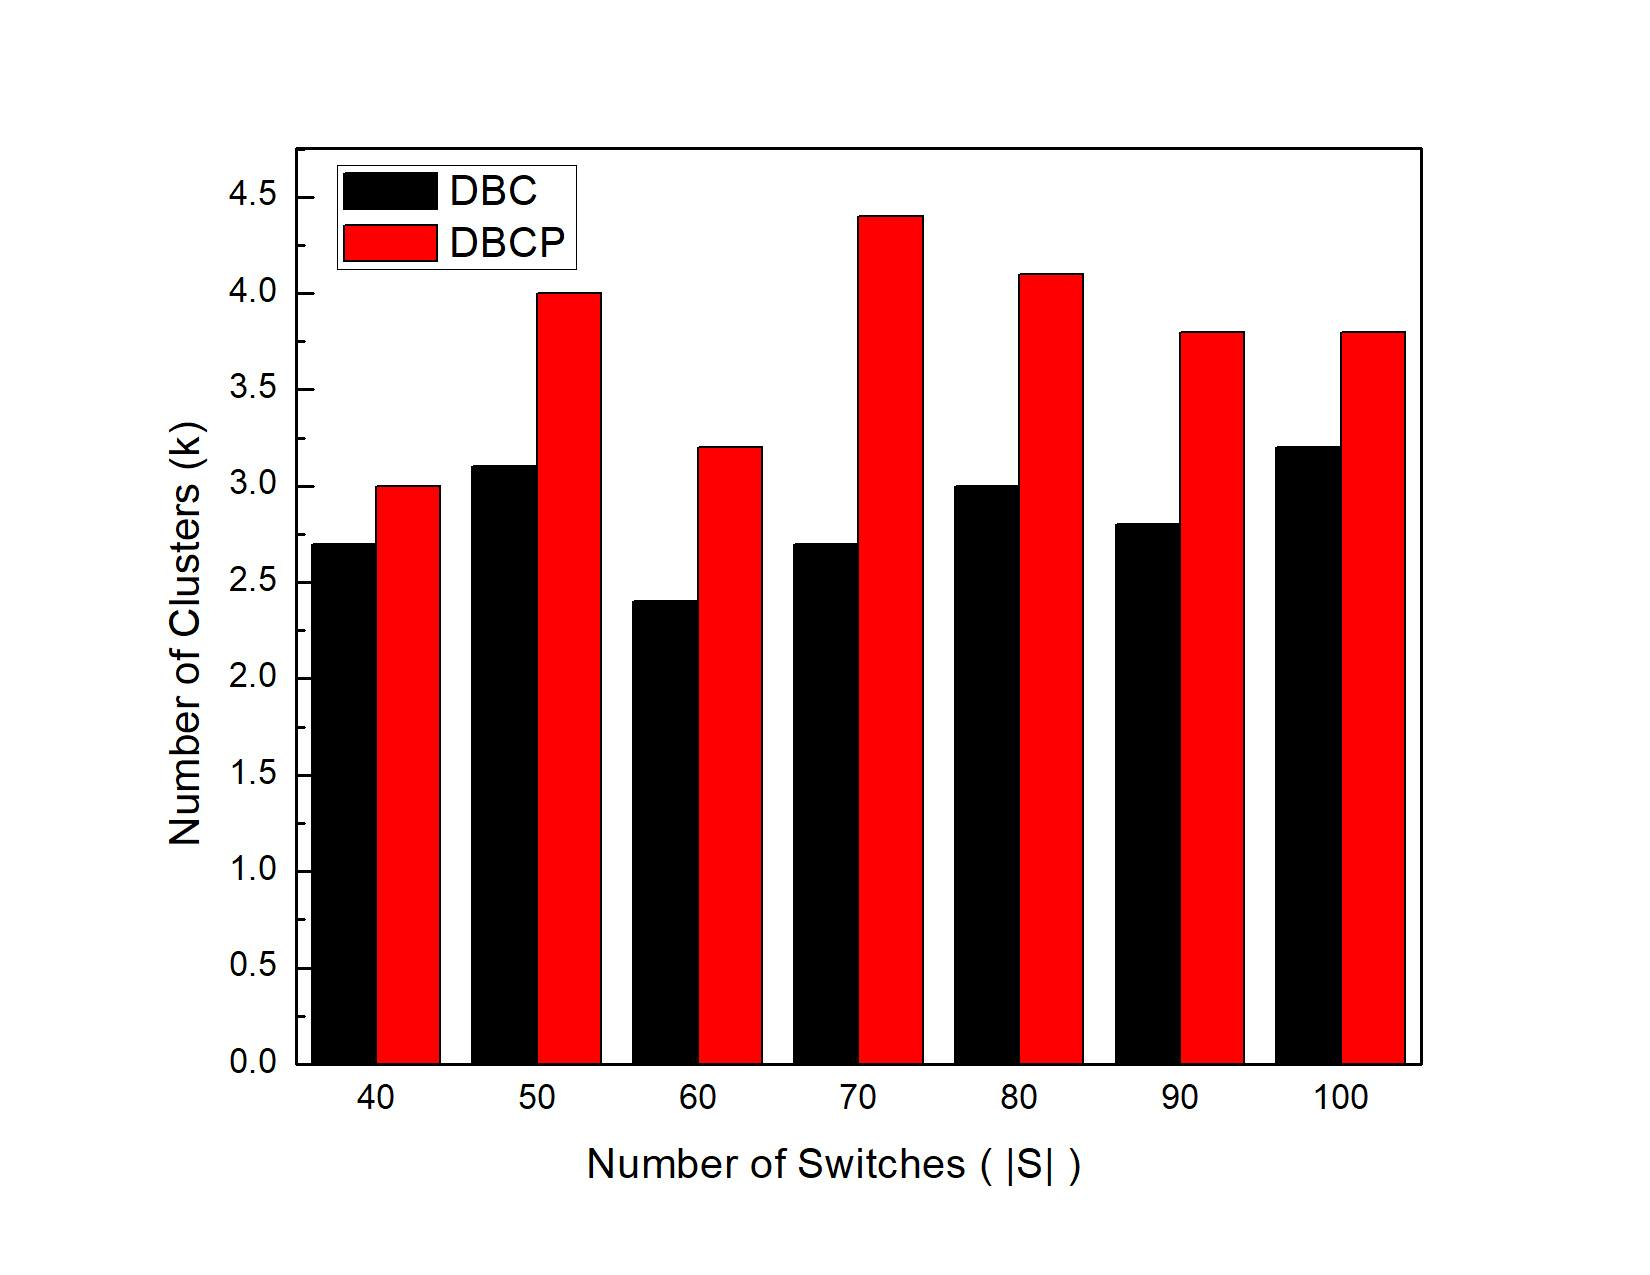
\includegraphics[width=\linewidth]{Figures/bar.jpg}
		\caption{Values of $k$ given by DBCP and DBC for different scenarios}
		\label{fig:barDiagram}
	\end{figure}
	\begin{figure}
		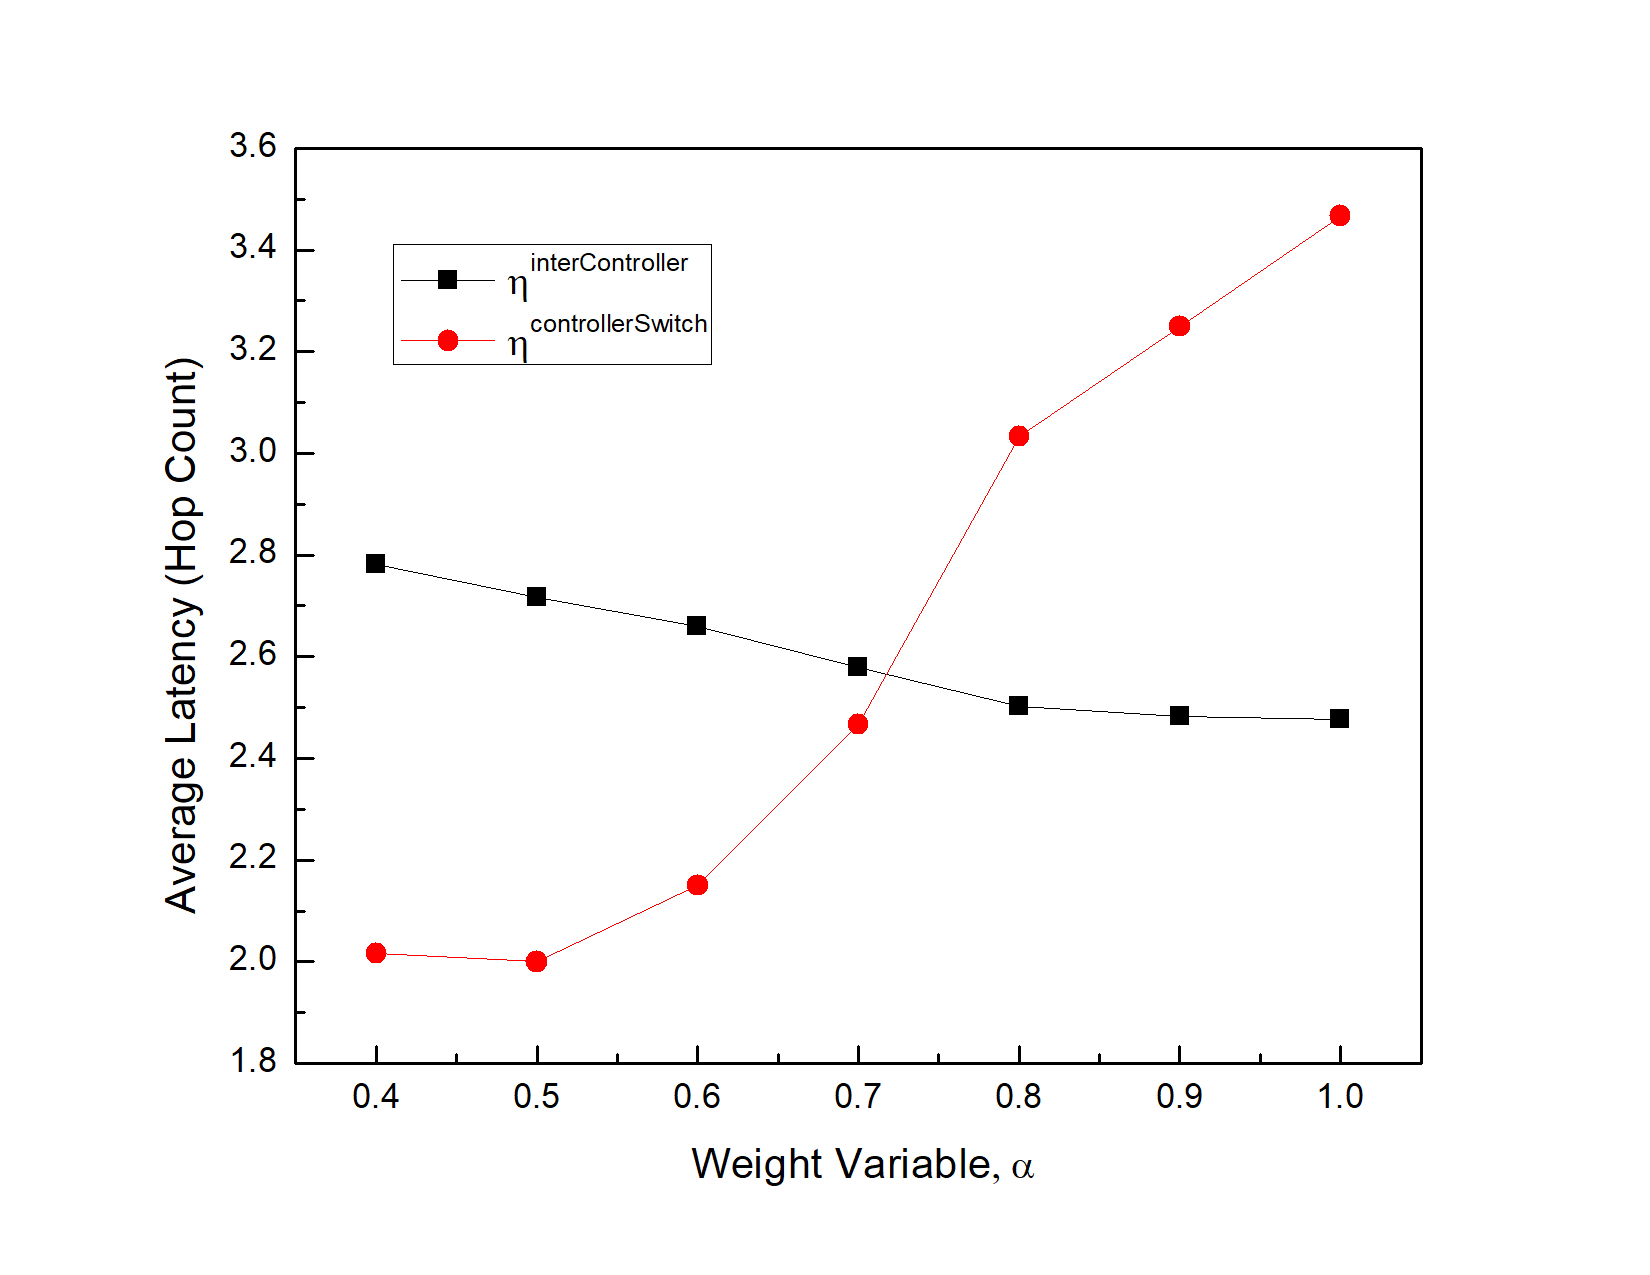
\includegraphics[width=\linewidth]{Figures/alphaGraph.jpg}
		\caption{Average controller-switch and controller-controller latency with respect to increasing weight variable, $\alpha$}
		\label{fig:alphaGraph}
		
		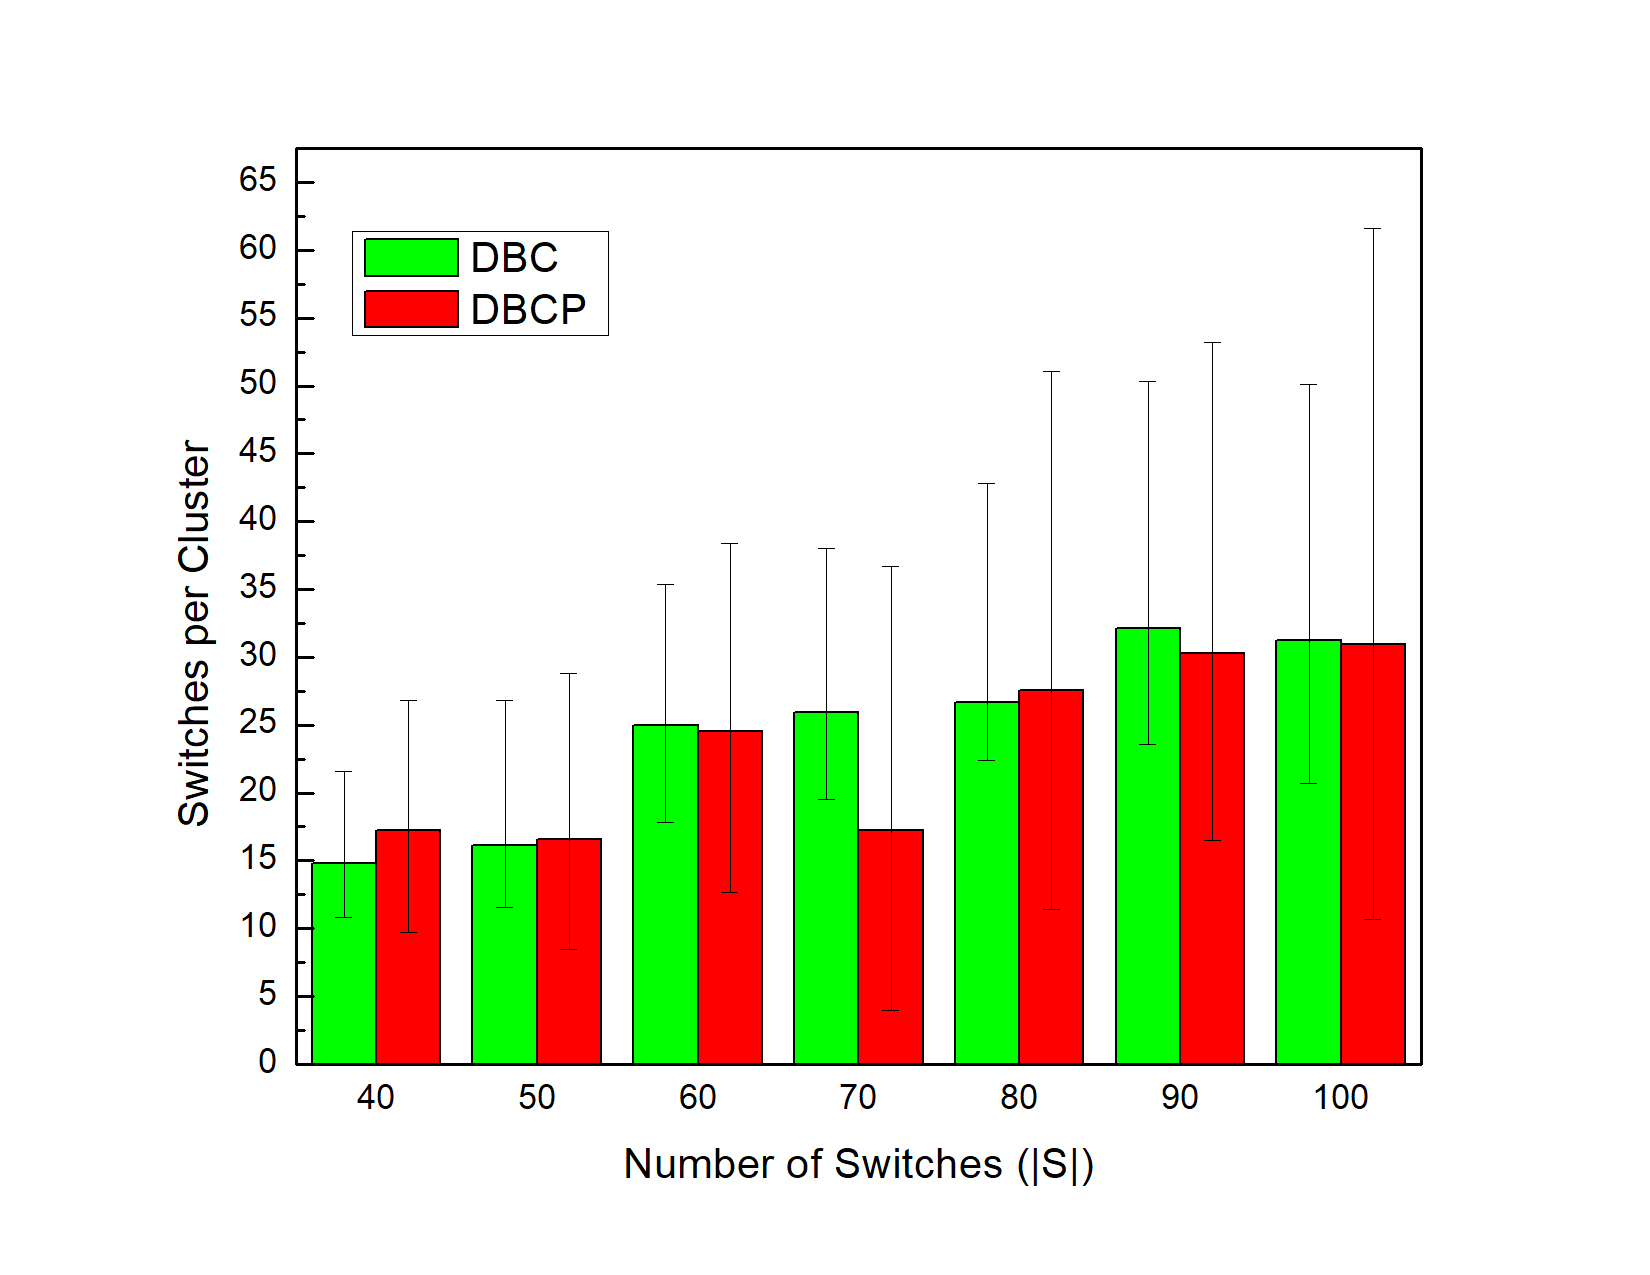
\includegraphics[width=\linewidth]{Figures/loadBalance.jpg}
		\caption{Comparison between DBCP and DBC in terms of average load per controller.}
		\label{fig:loadBalance}
		%	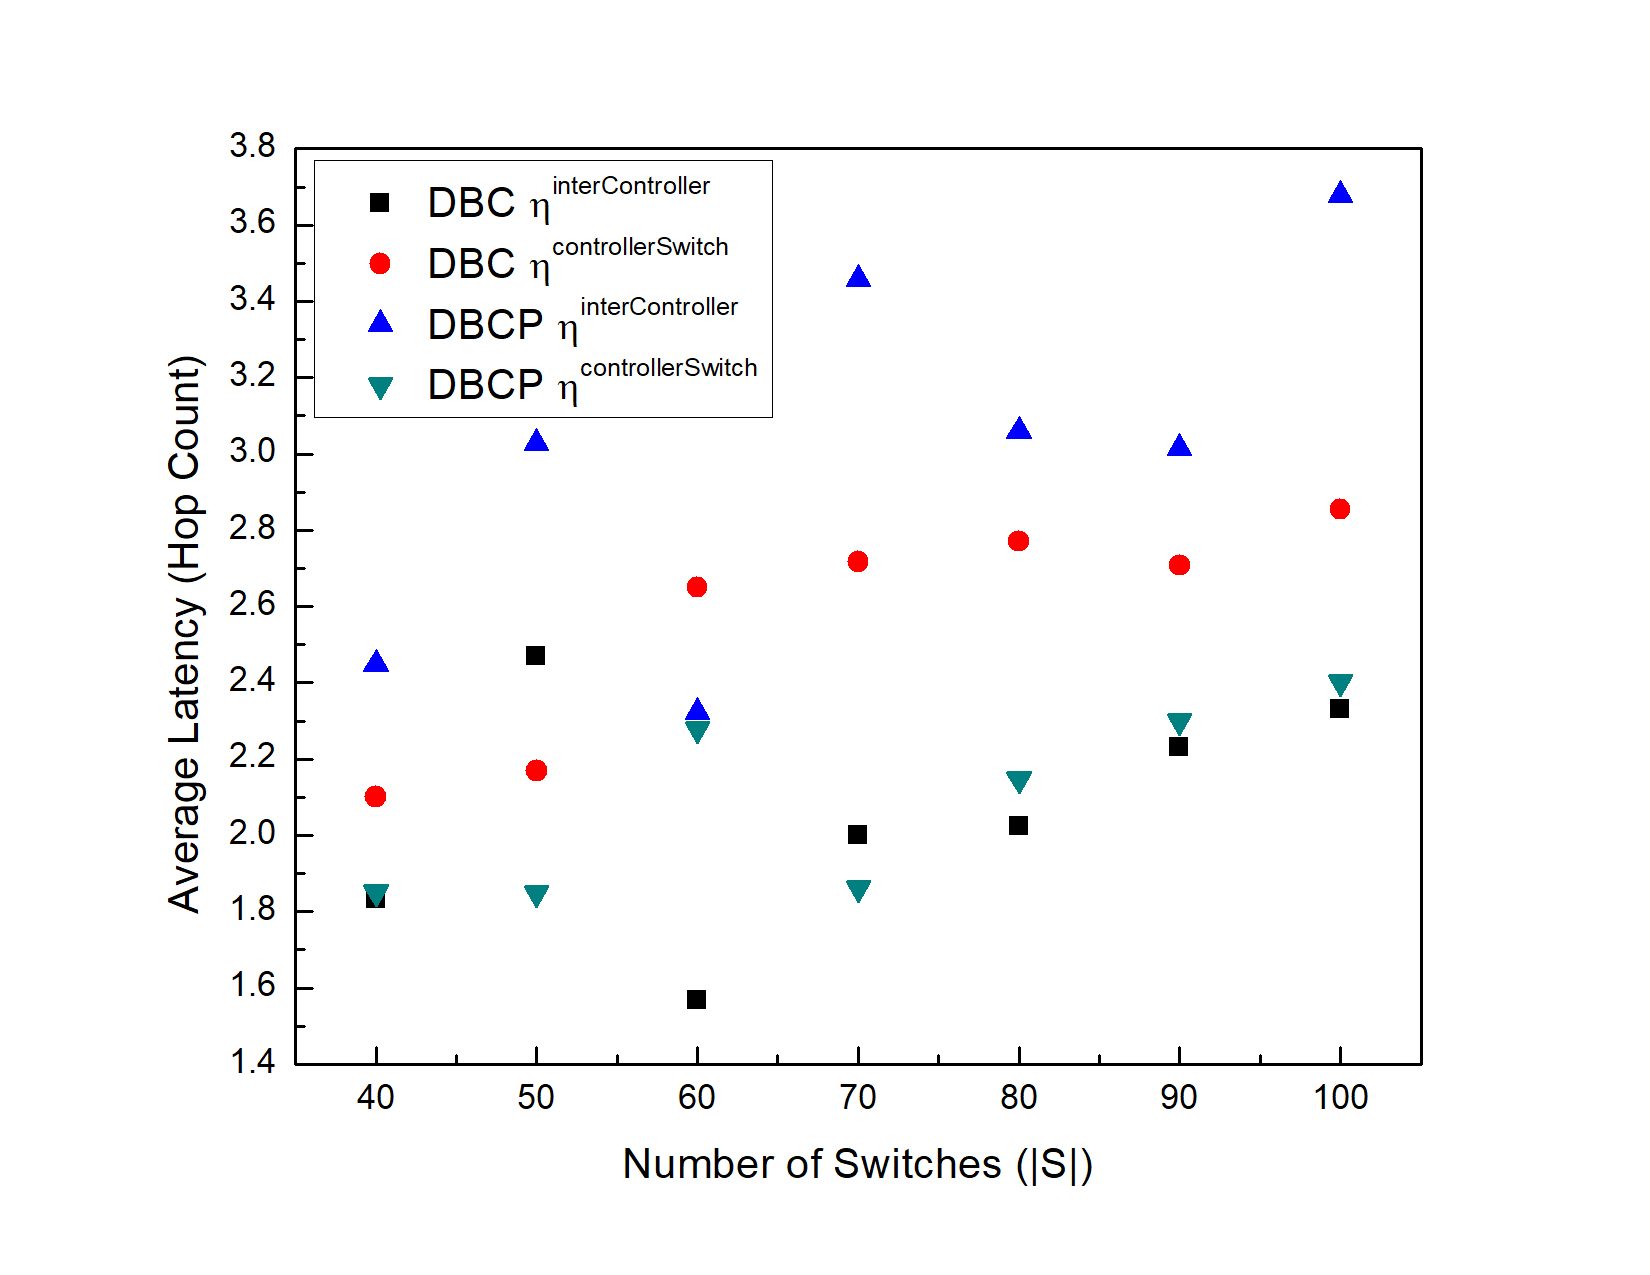
\includegraphics[width=\linewidth]{Figures/clusterGraph.jpg}
		%	\caption{Comparison between DBCP and DBC in terms of controller-switch and controller-controller latency}
		%	\label{fig:clusterGraph}
	\end{figure}
	We control the contribution of inter-controller latency and intra-cluster latency using a weight variable $\alpha$ (equation \ref{eqn:totlat}) which ranges from 0.0 to 1.0. When the value of $\alpha$ is increased, the intra-cluster latencies (equation \ref{eqn:controllerSwitch}) increase and the inter-controller latencies (equation \ref{eqn:interController}) decrease as presented in Fig. \ref{fig:alphaGraph}. When the value of $\alpha$ is set to $0.5$, inter-controller latencies are given priority by default, as the inter-controller distances are greater than intra-cluster distances. Our proposed algorithm outperforms DBCP in terms of inter-controller latency, however, DBCP gives better controller-to-switch latencies. We prioritize controller-to-controller latencies as control packets are essential in setting up new paths and conveying broken link information.
	
	In Fig. \ref{fig:loadBalance}, we compare the average, maximum, and minimum loads, of the controllers by adopting the number of switches per cluster which corresponds to the load of each controller. We observe that the deviation from the ideal load per controller in a balanced SDN ($|S|/k$), which can be calculated using equation \ref{eqn:deviation}, is higher for DBCP. Our proposed algorithm outperforms by forming clusters which are more balanced in terms of load per controller.
	
	\section{Conclusion} \label{conclusion}
	In this paper, we address the Controller Placement Problem (CPP) of SDN and propose a novel clustering algorithm named Degree-based Balanced Clustering (DBC). DBCP is a recent clustering algorithm which addresses the same research problem and minimizes overall setup latency of the SDN. Our proposed algorithm, DBC outperforms DBCP in terms of different latencies and balances the load of the controllers. We have shown that our algorithm has many advantages over other algorithms. DBC minimizes flow-setup latency and route synchronization latency through minimization of controller-to-switch and controller-to-controller distances. DBC creates balanced clusters with similar number of nodes and has polynomial time complexity.
	Our proposed algorithm can be extended to work on weighted networks which consider ongoing traffic of links and different delays like queuing delay in a congested network to intelligently select flow routes. The hop count can be replaced with average edge weights and the inter cluster separation updated accordingly. Future work can also include variable loads of switches and balance the cluster so that minimum load is imposed on each controller.
	
	\bibliographystyle{IEEEtran}
	\bibliography{bibFile}
\end{document}
